\chapter{Grundlagen}
\section{gRPC in Unity}
%Was ist das RPC Protokoll?
RPC steht für "Remote Procedure Call" (zu Deutsch: "Fernprozeduraufruf"). Es handelt sich um ein Protokoll und ein Konzept in der Informatik, das es ermöglicht, Funktionen oder Methoden auf entfernten Computern oder Prozessen aufzurufen, als ob sie auf dem lokalen Computer ausgeführt würden. RPC ermöglicht die Kommunikation zwischen verteilten Systemen und wird häufig in Client-Server-Anwendungen, Netzwerkdiensten und verteilten Systemen eingesetzt.\cite{Bengel.2004}\\

\begin{wrapfigure}{r}{0.25\textwidth} %this figure will be at the right
    \centering
    
\includegraphics[width=0.25\textwidth]{images/grpc-icon-color.png}
\end{wrapfigure}
Die Grundidee hinter RPC ist, dass ein Client-Programm eine Funktion oder Methode auf einem entfernten Server aufruft, als ob sie lokal vorhanden wäre. Der RPC-Mechanismus kümmert sich um die Details der Kommunikation, der Datenübertragung und der Rückgabewerte. Der Aufruf einer entfernten Funktion ähnelt daher stark einem normalen Funktionsaufruf in der Programmierung.\cite{Bengel.2004}\\

RPC erleichtert die Entwicklung von verteilten Anwendungen, da Entwickler sich nicht um die Details der Netzwerkkommunikation kümmern müssen. Es gibt verschiedene RPC-Implementierungen und Protokolle, darunter gRPC, XML-RPC, JSON-RPC und andere, die in verschiedenen Umgebungen und Anwendungsfällen eingesetzt werden können.\cite{Bengel.2004}\\

%Was ist gRPC?

gRPC ist ein leistungsstarkes Remote Procedure Call (RPC)-Framework, das von Google entwickelt wurde. Es wird häufig in verteilten Systemen und Microservices-Architekturen verwendet, um die Kommunikation zwischen verschiedenen Diensten zu erleichtern.\\

Eine der herausragenden Eigenschaften von gRPC ist die Verwendung des HTTP/2-Protokolls als Transportmechanismus. HTTP/2 bietet signifikante Verbesserungen gegenüber HTTP/1.x, darunter die Möglichkeit, mehrere Anfragen und Antworten über eine einzige TCP-Verbindung zu multiplexen, Header-Komprimierung und verbesserte Leistung.\\

Ein weiterer großer Vorteil von gRPC ist seine plattformübergreifende Unterstützung. Es ist in einer Vielzahl von Programmiersprachen verfügbar, darunter C++, Java, Python, Go, Ruby, C\# und mehr. Dies ermöglicht die Entwicklung von Client- und Serveranwendungen in verschiedenen Sprachen, die miteinander kommunizieren können.\\

Um Schnittstellen und Datenstrukturen eindeutig und plattformübergreifend zu definieren, verwendet gRPC die Protobuf (Protocol Buffers)-Sprache als IDL (Interface Definition Language). Diese starke Typisierung ermöglicht es Client und Server, genau zu wissen, welche Daten erwartet werden, ohne auf textbasierte Formate wie JSON oder XML angewiesen zu sein.\\

Eine weitere Stärke von gRPC ist die Unterstützung von bidirektionaler Streaming-Kommunikation. Das bedeutet, dass sowohl der Client als auch der Server Daten gleichzeitig senden und empfangen können, was für Anwendungsfälle wie Chat-Anwendungen oder Echtzeit-Spiele sehr nützlich ist.\\

Die Authentifizierung und Sicherheit sind ebenfalls integrale Bestandteile von gRPC. Es bietet Funktionen zur Authentifizierung und Verschlüsselung, um die Kommunikation zwischen Client und Server sicher zu gestalten. Unterschiedliche Authentifizierungsmechanismen wie OAuth, JWT und TLS werden unterstützt.\\

Ein weiterer Vorteil von gRPC ist die automatische Codegenerierung. Auf Grundlage der in Protobuf definierten Schnittstellen und Nachrichten generiert gRPC automatisch Client- und Servercode, was die Entwicklung und Wartung von gRPC-Anwendungen erleichtert.\\

Insgesamt bietet gRPC eine effiziente und plattformübergreifende Möglichkeit, die Kommunikation zwischen verschiedenen Komponenten in verteilten Systemen zu verwalten. Es wird in einer Vielzahl von Anwendungen eingesetzt, von Mikrodiensten-Architekturen über IoT-Geräte bis hin zu Cloud-basierten Anwendungen.\\

%Wie funktioniert das gRPC Protokoll in Unity?

\begin{wrapfigure}{l}{0.25\textwidth} %this figure will be at the right
    \centering
    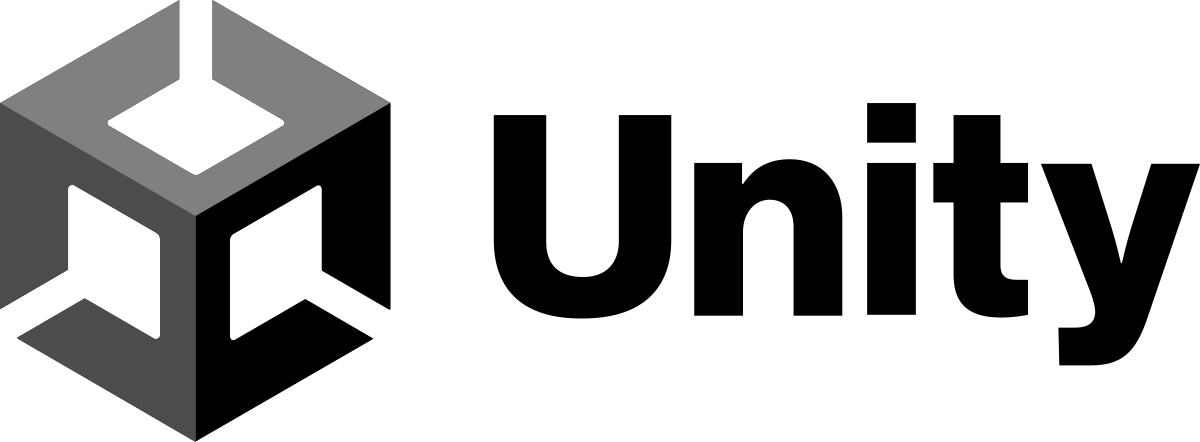
\includegraphics[width=0.25\textwidth]{images/Unity_2021.svg.png}
\end{wrapfigure}

In Unity ist gRPC eine Implementierung des gRPC-Frameworks, das speziell für die Verwendung in Unity-Projekten entwickelt wurde. Es ermöglicht die Integration von gRPC-Kommunikation in Unity-Anwendungen, um die Interaktion zwischen Unity-Anwendungen und entfernten Servern oder Diensten zu erleichtern.\\

Die Verwendung von gRPC in Unity erfordert in der Regel die Integration von gRPC-Paketen oder -Bibliotheken in Ihr Unity-Projekt sowie die Erstellung von gRPC-Clientcode, um Serveraufrufe durchzuführen. Dadurch können Unity-Entwickler die Vorteile von gRPC nutzen, um die Kommunikation mit Servern oder Diensten in ihren Spielen oder Anwendungen zu vereinfachen und zu optimieren.\\

\section{Thales Framework}
%Was ist Thales?
Die Virtualisierung von Anwendungen mittels Modellierung und Simulation eröffnet eine Vielzahl von Vorteilen gegenüber der Verwendung physischer Anwendungen. Diese Vorteile erstrecken sich auf verkürzte Entwicklungszyklen und eine gesteigerte Zuverlässigkeit der Anwendungen. In diesem Kontext strebt das Thales-Framework an, eine effiziente Plattform bereitzustellen, welche es den Anwendern ermöglicht, ihre eigenen virtuellen Anwendungen auf effektive Weise zu entwickeln.\\

Ein zentrales Ziel von Thales besteht darin, Werkzeuge zur zügigen und effizienten Erstellung von Anwendungsmodellen zur Verfügung zu stellen. Dies wird durch die Umsetzung eines Gemeinschafts- und Paket-basierten Ansatzes ermöglicht, wobei Artifactory als Paketregister fungiert. Diese Herangehensweise erleichtert die rasche gemeinsame Nutzung von Modellressourcen innerhalb der gesamten Anwendergemeinschaft.\\

Thales nutzt zur Erreichung hoher Simulationseffizienz und -genauigkeit Sensormodelle, welche von Grafikprozessoren (GPUs) unterstützt werden.\\

Durch die Anwendung von Protobuf und gRPC wird die Integration in unterschiedliche Programmiersprachen und Plattformen ermöglicht. Auf diese Weise ist der Zugriff auf die Anwendung über diverse Programmiersprachen und Plattformen hinweg realisierbar. \\

Des Weiteren gestaltet sich die Erweiterung von Thales durch Unity-Pakete als unkompliziert.\\

Ein weiterer hervorstechender Aspekt in der Entwicklung von Thales ist die Minimierung des Eigenentwicklungsanteils durch die verstärkte Nutzung existierender Bibliotheken und Tools. Dieser Ansatz trägt zur Effizienzsteigerung bei der Umsetzung des Frameworks bei.\cite{.02.09.2023}\\

\begin{figure}[htp]
    \centering
    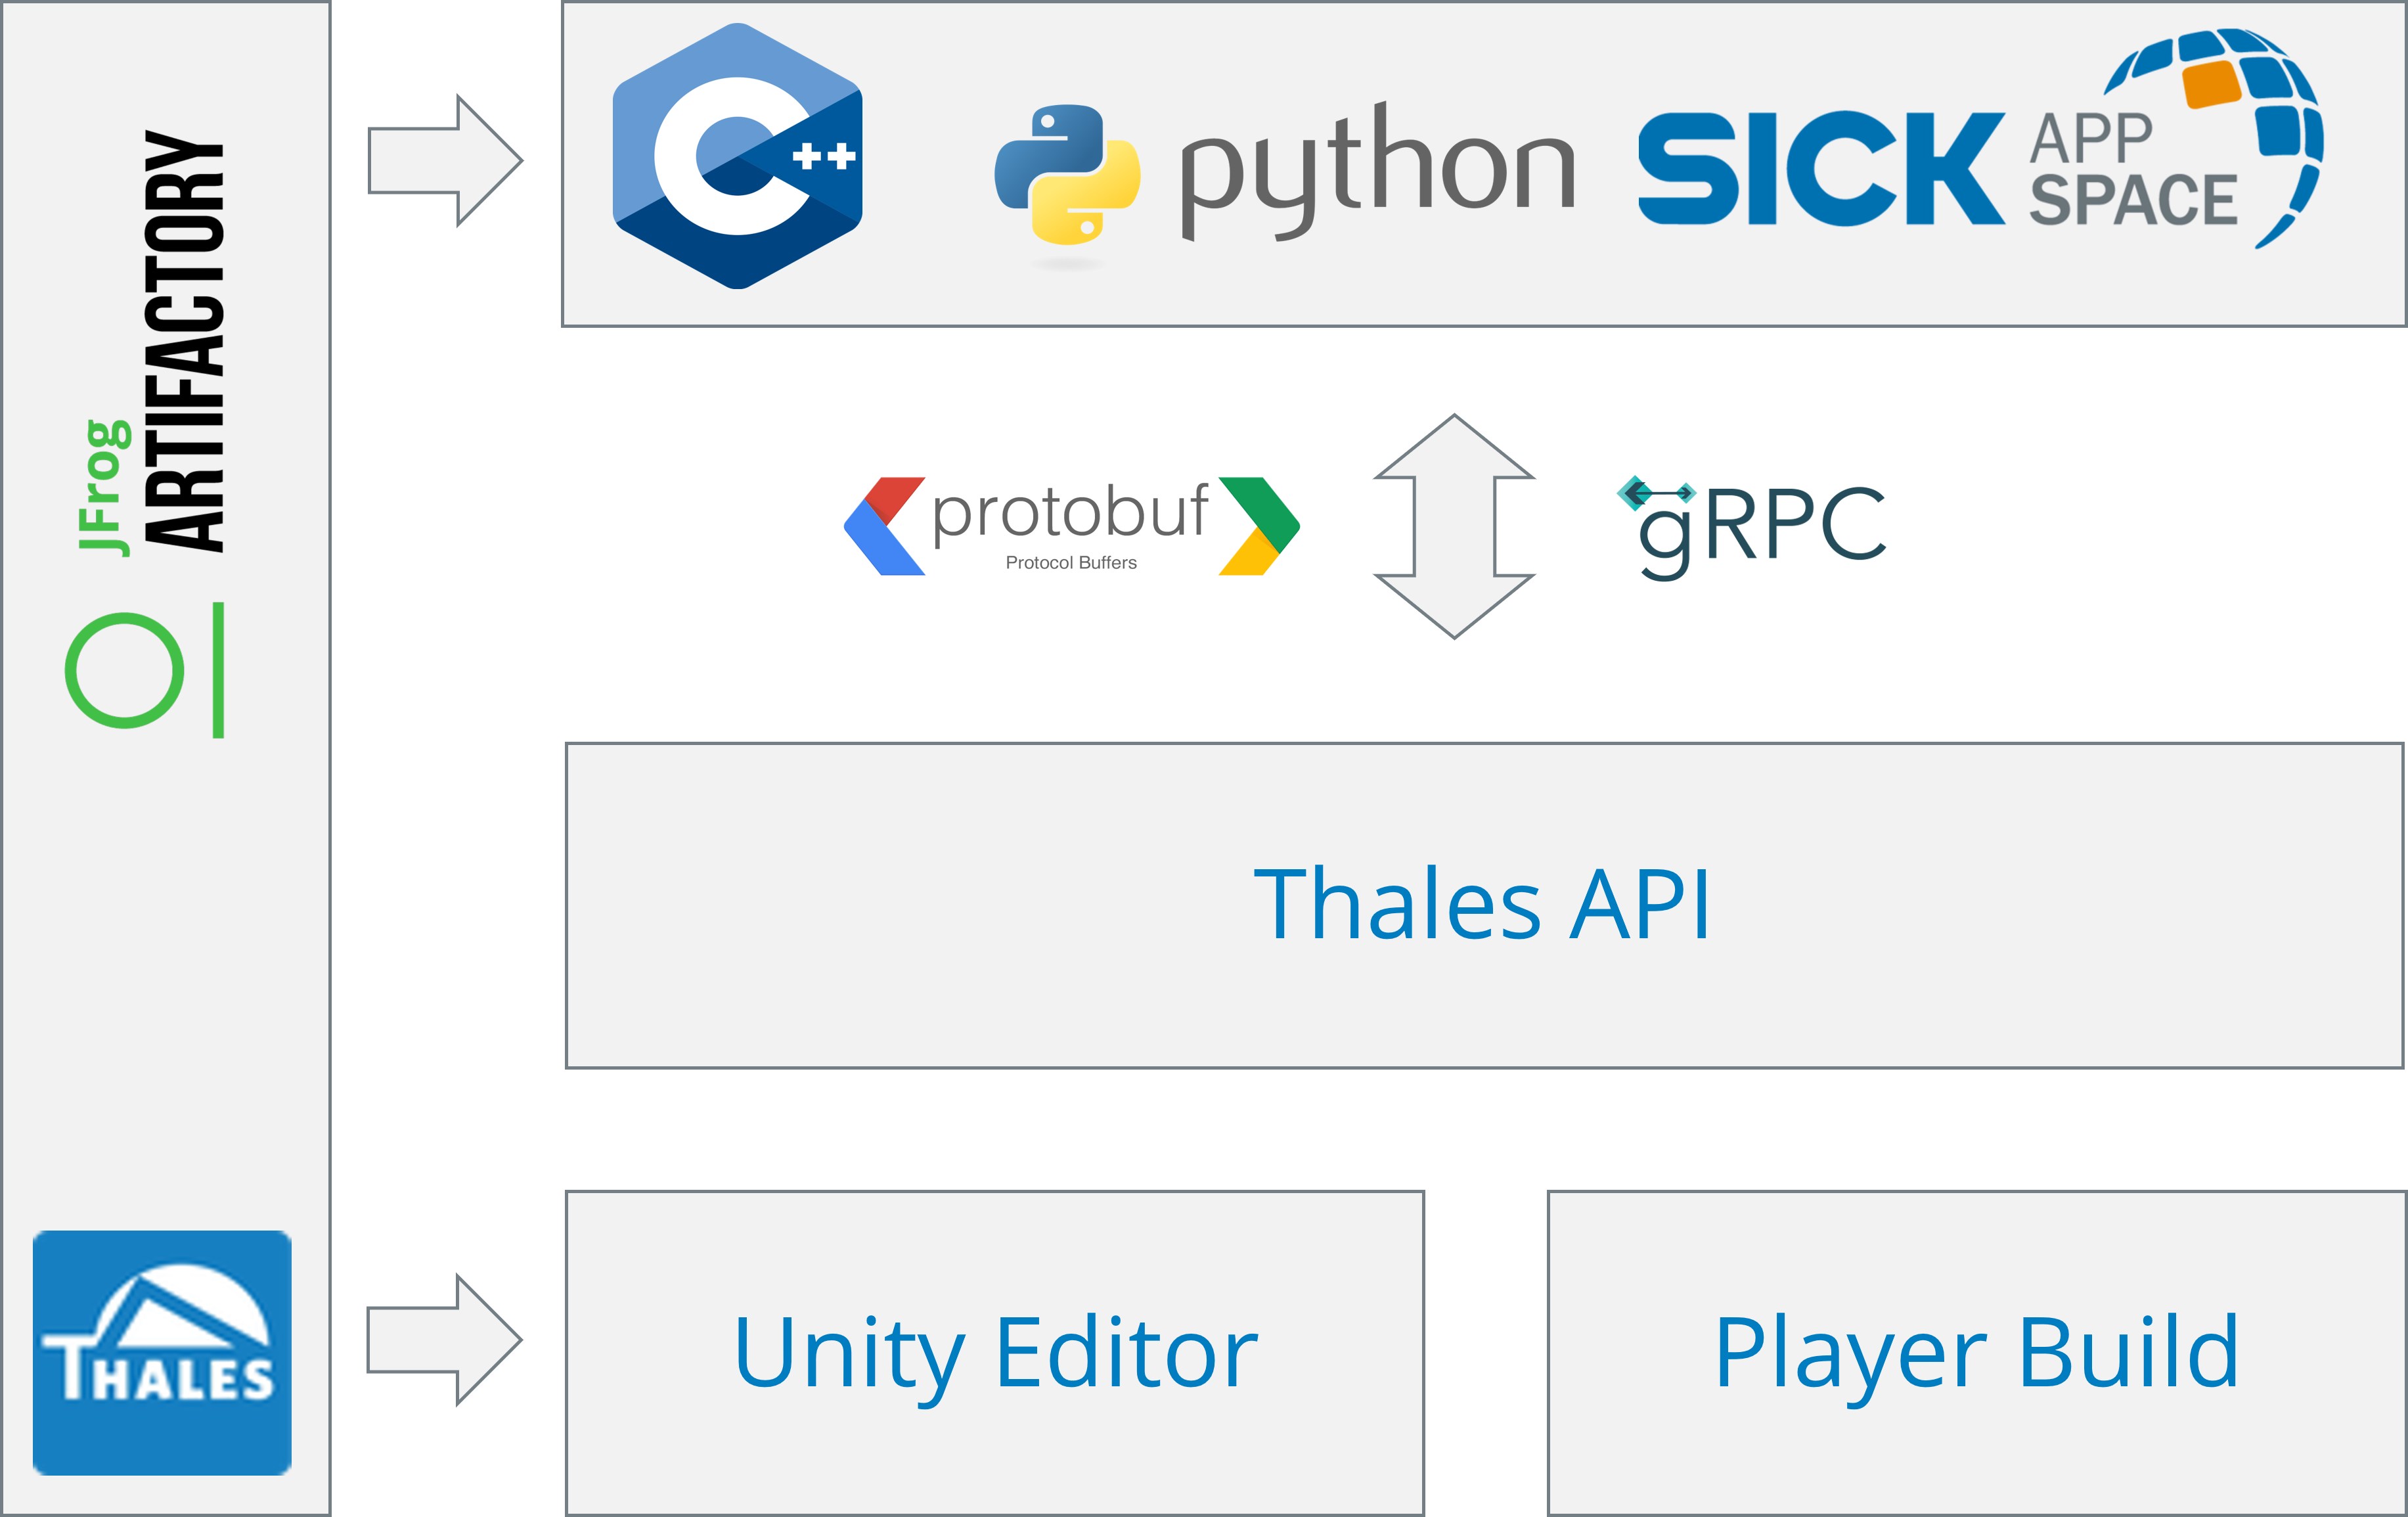
\includegraphics[width=(\textwidth/2)]{images/Thales_Framework.png}
    \caption{Thales Framework}
    \label{fig:Thales-Framework}
\end{figure}


\section{Senoren in der VirtuellenUmgebung}
%Wie funktionieren die Sensoren in Unity?
Im Thales-Paket sind vordefinierte LIDAR-Scanner als Fertigteile enthalten, die mühelos in der entsprechenden Szene instanziiert werden können. Alternativ besteht die Möglichkeit, einen generischen LIDAR-Scanner zu erstellen und entsprechend zu konfigurieren, indem die Systemdiagrammkomponente direkt genutzt wird. Die Nutzung von vorgefertigten Elementen, wie in der Sektion "Spezifische LIDAR-Prefabs" dargestellt, bietet eine zügige und unkomplizierte Möglichkeit, die Arbeit mit virtuellen LIDAR-Sensoren aufzunehmen. Dies erweist sich insbesondere dann als hilfreich, wenn der gewünschte Sensor bereits in Thales verfügbar ist. Falls die Absicht besteht, LIDAR-Scanner zu verwenden, die nicht im bereitgestellten Paket enthalten sind, oder wenn generell LIDAR-Geräte in einem frühen Entwicklungsstadium erforscht werden sollen, bietet es sich an, die generische LIDAR-Scanner-Komponente zu nutzen. Für Fälle, in denen eine raffiniertere Sensormodellierung angestrebt wird, besteht sogar die Möglichkeit, eine individuelle Systemdiagrammkomponente zu erstellen. Referenzimplementierungen hierzu sind in den Systemgraph-Komponenten innerhalb von Thales verfügbar.\\

\begin{figure}[htp]
    \centering
    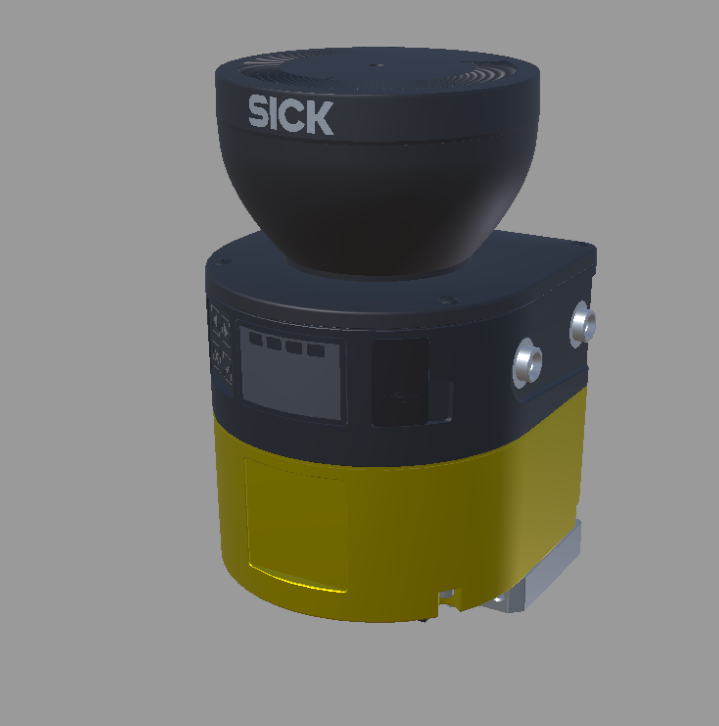
\includegraphics[width=(\textwidth/3)]{images/ModelMircoScan.PNG}
    \caption{MicroScan3}
    \label{fig:MicroScan3}
\end{figure}

\subsubsection*{Rasterisierung basierende LIDAR-Scanner}



Diese Implementierung nutzt Rasterisierungs-Shader als Backend-Technologie und erfordert keine RTX-Hardware. Obwohl es in gewisser Hinsicht seine Grenzen hat, ist es oft eine vernünftige Wahl, insbesondere wenn Sie keine hohe Simulationsgenauigkeit benötigen.\\

\begin{figure}[htp]
    \centering
    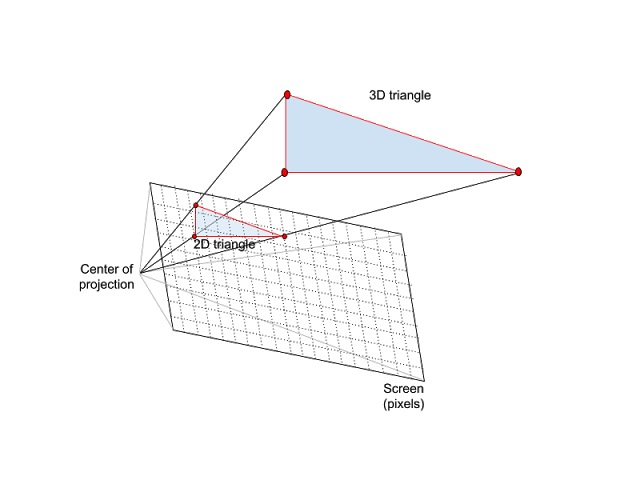
\includegraphics[width=(\textwidth/2)]{images/projection_3d_to_screen.png}
    \caption{Rasterisierung}
    \label{fig:Rasterisierung}
\end{figure}


Bei der Rasterisierung werden die Objekte auf dem Bildschirm aus einem Netz virtueller Dreiecke oder Polygone erstellt, die 3D-Modelle von Objekten bilden. In diesem virtuellen Netz überschneiden sich die Ecken jedes Dreiecks - die so genannten Scheitelpunkte - mit den Scheitelpunkten anderer Dreiecke unterschiedlicher Größe und Form. Jedem Scheitelpunkt ist eine Vielzahl von Informationen zugeordnet, darunter seine Position im Raum sowie Informationen über Farbe, Textur und seine "Normale", mit der die Ausrichtung der Oberfläche eines Objekts bestimmt wird.\\
%https://de.wikipedia.org/wiki/Rasterung#:~:text=In%20der%202D%2DComputergrafik%20bezeichnet,einer%20Vektor%2D%20in%20eine%20Rastergrafik. Teile davon kopieren wenn noch Zeit ist
%Wie funktioniert die Raterisierung in diesem Kontext?
%Die Kamera nimmt ein Bild auf und skalliert es runter auf bis aus den Vector grafiken nur noch Pixel zusehen sind. Mit dem Abstand der Pixel kann die Distanz bestimmt werden. so habe ich das verstanden

\begin{figure}[htp]
    \centering
    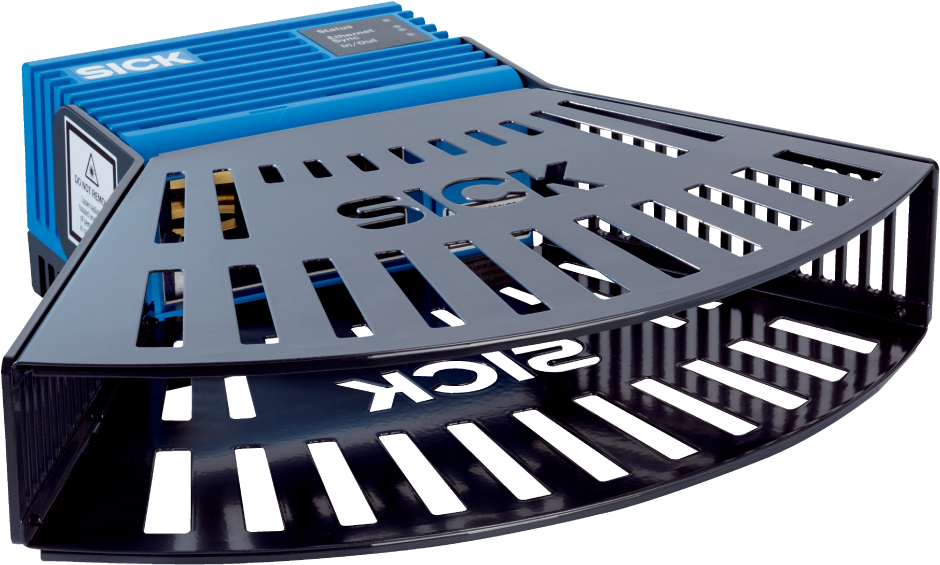
\includegraphics[width=(\textwidth/3)]{images/LMS4000.png}
    \caption{LMS4000}
    \label{fig:LMS4000}
\end{figure}
\subsubsection*{RTX basierende LIDAR-Scanner}
Das RTX-basierte Lidar-Scanner-Modell nutzt Echtzeit-Raytracing und erfordert daher eine Grafikkarte, die RTX unterstützt. Diese Implementierung kann erhalten werden, indem das GenericLidarScannerRTX-Systemdiagramm auswählt wird.\\





%Wie funkt RTX raytracing?
%Es basiert auf raytracing so wie in der realen welt fällt licht auf das object und dann in auf den Sensor so kann der Abstand durch time of light bestimmt werden.
